\documentclass[hidelinks, 12pt, oneside]{article}
\usepackage{bookmark}
\usepackage{graphicx}
\usepackage{hyperref}
\usepackage{titlesec}
\setcounter{secnumdepth}{4}
\usepackage[utf8]{inputenc}
\usepackage[english]{babel}
\usepackage{color}


\begin{document}

	\begin{center}
    \centering
    
%University logo
    
\includegraphics[width=144px]{img/icon.png}
    \rule{0\linewidth}{0.15\linewidth}\par
    
    		\begin{center}
		{\uppercase{\Large User Manual\par}}
   		{\Large iCrawler \par}
   			\vspace{1cm} 
   		{\Large Emilio Mumba  \par} 
    		\vspace{1cm}
		   		
    		{\Large The 5 Concurrent Nodes \par} 
    		\vspace{1cm}
		
		{\normalsize Khathutshelo Shaun Matidza\par}
		{\normalsize Sylvester Sandile Mpangane\par}
		{\normalsize Thabang Michael Letageng\par}
		{\normalsize Matthew Nel\par}
		
		\end{center}

		\textbf{}		
		\centering
		\vspace{2cm}
		Department of Computer Science, University of Pretoria

		
	 	{\Large  September 2015}
\end{center}
\clearpage


	\tableofcontents
	\newpage
	
	\section{Overview}
	\emph{You have a 13 year old child whom in the past years excelled at school in academics and sports activities. Suddenly, out of the blue, you start noticing a change in his behavior; his/her grades are dropping, he/she spends more time alone and doesn’t enjoy doing the things he/she use to do. This can be really stressful and saddening for any parent/guardian; even worse, when the child is not talking to you...}
	he/she could be a victim of bullying, he/she could be associated with bad company, or it could be a temporal thing. \textbf{Where do you start}?
	\newline
	 
	 \uppercase{What is \MakeLowercase iCrawler?}
	 \begin{flushleft}
	 iCrawler is a mobile monitoring app that monitors crucial activities on android mobile devices.	
	The app uses the most efficient methods to collect and report the data to a dashboard.
	The user can then login, from anywhere in the world, and view the reported data.
	\end{flushleft}
	
	\uppercase{Why choose\MakeLowercase iCrawler?}
	 \begin{flushleft}
	 The app is designed with the parent and child in mind. Unlike any other mobile monitoring app, the app is not designed for multi-purpose use, instead it is strictly focused on the parent and child. It makes use of highly efficient and reliable methods to collect the data without exhausting the devices limited resources. Extensive research was done in the technology used in the development. Through this the app and dashboard can be ranked with most, if not all, the current trending competitors.
	\end{flushleft}
	
	\uppercase{\MakeLowercase iCrawler? features}
	 \begin{flushleft}
	 Call logging (incoming,outgoing, and missed)\newline
	SMS logging (sent,received)\newline
	Web monitoring (history)\newline
	Wi-Fi connections (name, MAC)\newline
	Installed apps (Facebook, Angry Birds, etc)\newline
	User geolocation (last seen)\newline
	Mobile device on/off
	\end{flushleft}
	\newpage
	
	
	\section{Configuration}
	
	\begin{tabular}{ |l|l| }  \multicolumn{2}{|c|}{
\includegraphics[width=0.1 \textwidth]{img/icon.png}iCrawler}
	 \\ \hline\noalign{\smallskip} \textbf{Stable release} & 1.0
	  \\\\ \noalign{\smallskip} \textbf{Development status}& Active
	  \\\\ \noalign{\smallskip}\textbf{Operating System}& Android 4.2+
	  \\\\ \noalign{\smallskip}\textbf{Platform}& Android
	  \\\\ \noalign{\smallskip}\textbf{Internet connection} & Yes
	  \\\\ \noalign{\smallskip}\textbf{Available in} & English
	  \\\\ \noalign{\smallskip}\textbf{Type}& Monitoring Application
	  \\\\ \noalign{\smallskip}\textbf{License}& Free
	  \\\\ \noalign{\smallskip}\textbf{Website}& www.github.com/u11241617/COS301-Mobile-Monitoring-App
	  %\hline
	 \end{tabular}\newpage
	%%%%%%%%%%%%%%%%%%%%%%%%%%%%%%%%%%%%%%%%%%%%%%%%%%%%%%%%%%%%%%%%%%%%%%%%%%%%%%%%%%%
	\section{User Access Levels}
		Our Github repository is private, only invited users can download the appliaction, additionaly a user has  to be registered on iCrawler to be able to have the app submit their user activities onto the dashboard, and to be able to log onto the dashboard.\newline
	\section{Installation}
	The iCrawler APK (Android Application Kit) is currently only available for download on our GitHub repository. Follow this link inorder 
	to start the download\dots\newline
		\href{url}{https://github.com/u11241617/COS301-Mobile-Monitoring-App/tree/master\\/Android\%20Project/}\\
		\emph{NB:} Open the \emph{app-release} folder to find the apk \newline \newline
		When the download has successfully completed the installation should automatically start, if not follow the following steps:\newline
	  
	 \begin{enumerate}
 	 	\item Navigate to 'File Management' from the options menu on your device
 	 	\item Under the 'Download' folder locate and launch a file named 'iCrawler.apk' within this folder
 	 	\item When a 'Install blocked' popup appears, select the 'Settings' option
 	 	\item Scroll down and check the option 'Unknown Sources'
 	 	\item Another popup will appear, simply click 'OK' then 'Next' followed by 'Install'
 	 	\item On completion you will see the options 'Done' and 'Open', click 'Open' to start the app \ldots
 	\end{enumerate}\newpage


	\section{Getting Started}
	After successful installation, locate the iCrawler app icon and click on it to launch the app.
	 \begin{figure}[h!]
	 	 \caption{Launching iCrawler app}
	 	 \centering 																																	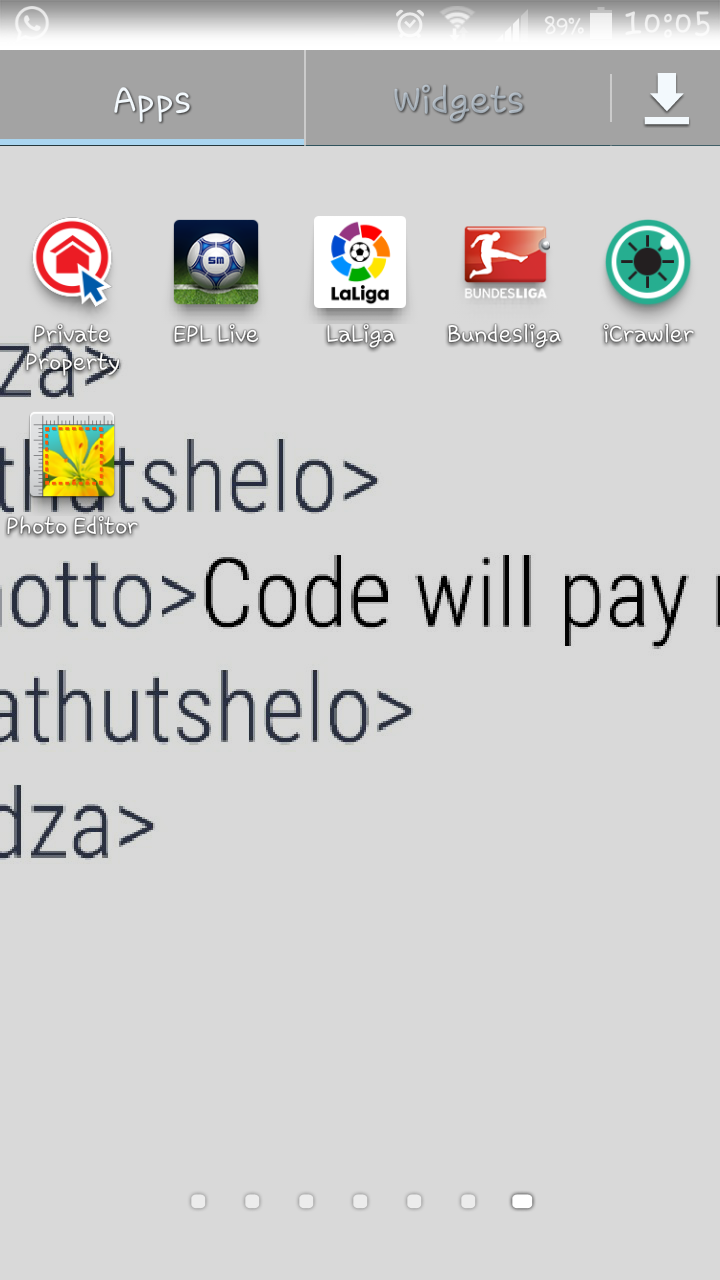
\includegraphics[width=0.5 \textwidth]{img/newImgs/appLaunch.png}
	 \end{figure}\newpage
	 
	 \begin{itemize}
	 	\item \textbf{Welcome to iCrawler}\newline
	 	This is the landing page when you launch the app. This page introduces what the app is about and also provides you
	 	with the options to either proceed with the app tour or skip to sign up/sign in.
	 	 
	 	 %Welcome page%
	 	 \begin{figure}[h!]
	 	 	\caption{Welcome to iCrawler}
	 	 	\centering 																																		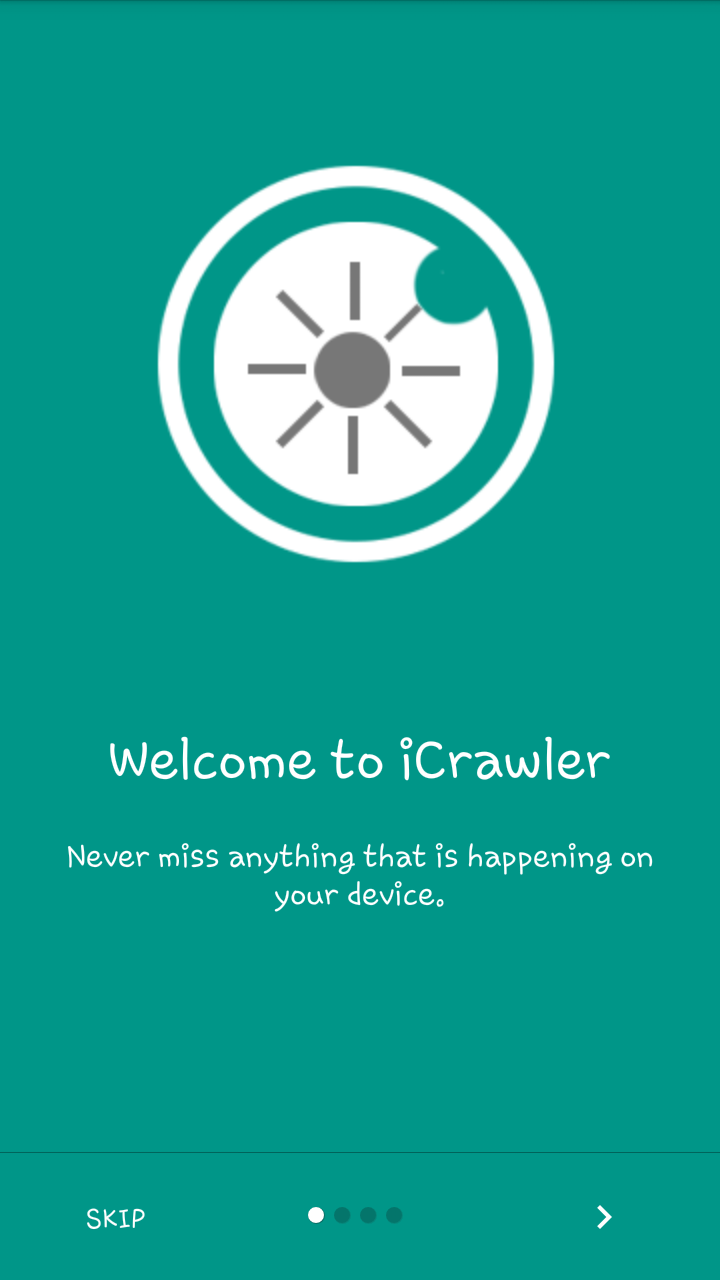
\includegraphics[width=0.5 \textwidth]{img/newImgs/landingPage.png}
	 	 \end{figure}\newpage
	 	 
		\item \textbf{Take tour}\newline
	 	If you opt to take a tour, this tour will explain all the features that come with this app.\newline\newline
	 	The app runs on the background collecting and compiling data logs of activities on your device. 
	 	 
	 	 %tourpage one%
	 	 \begin{figure}[h!]
	 	 	\caption{Never left alone}
	 	 	\centering 																																		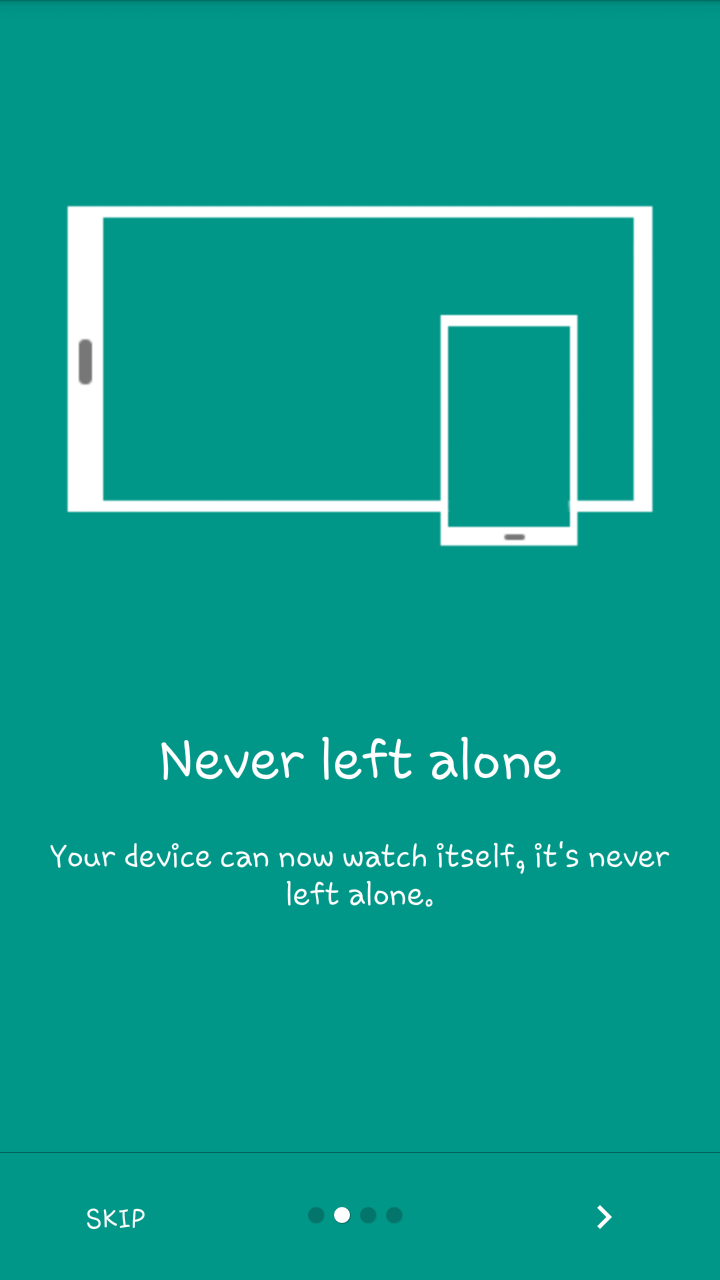
\includegraphics[width=0.5 \textwidth]{img/newImgs/tourOne.png}
	 	 \end{figure}\newpage	
	 	 
	 	 To view the compiled logs you simply log onto the web application, using either your laptop or desktop, with your credentials and 
	 	 view the collected data. 
	 	 %tourpage two%
	 	 \begin{figure}[h!]
	 	 	\caption{View monitored logs}
	 	 	\centering 																																		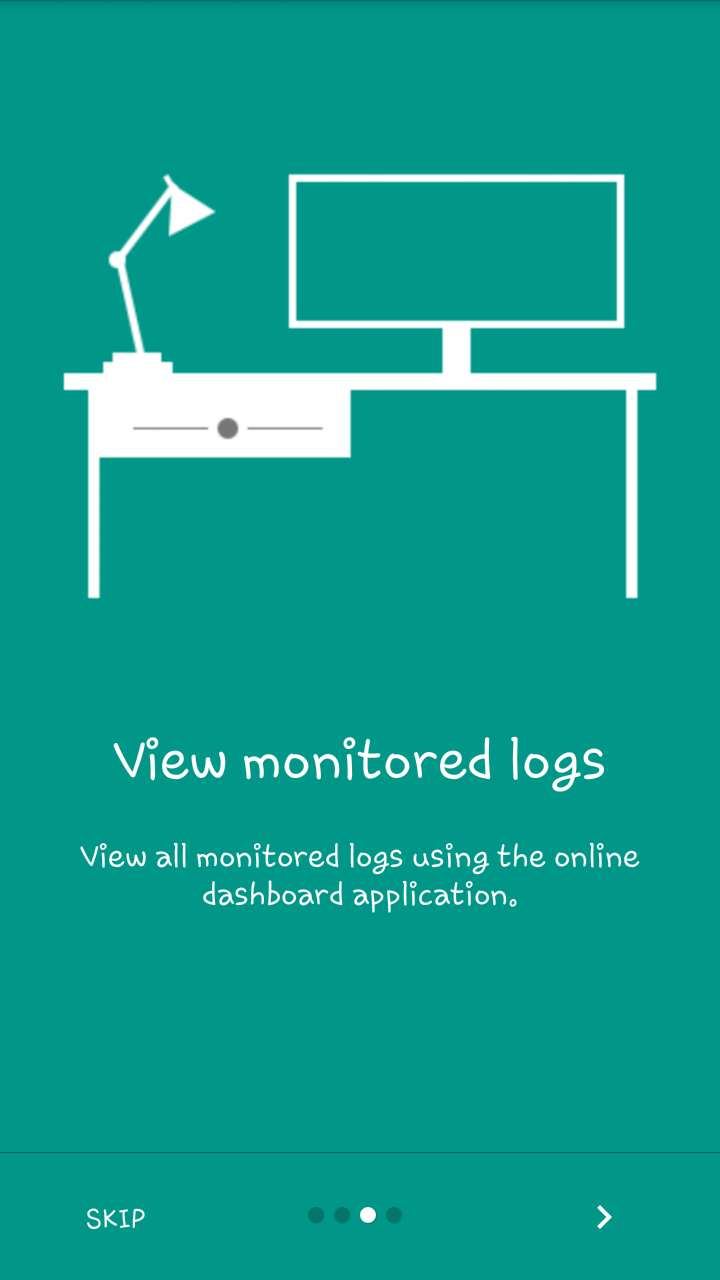
\includegraphics[width=0.5 \textwidth]{img/newImgs/tourTwo.png}
	 	 \end{figure}\newpage	 	 
	 	 
	 	 To be able to use the awesome features that come with this app, all you have to do is sign up, if you are a new user, or simply
	 	 just sign in and you are ready to go! 
	 	 %tourpage three%
	 	 \begin{figure}[h!]
	 	 	\caption{All you have to do}
	 	 	\centering 																																		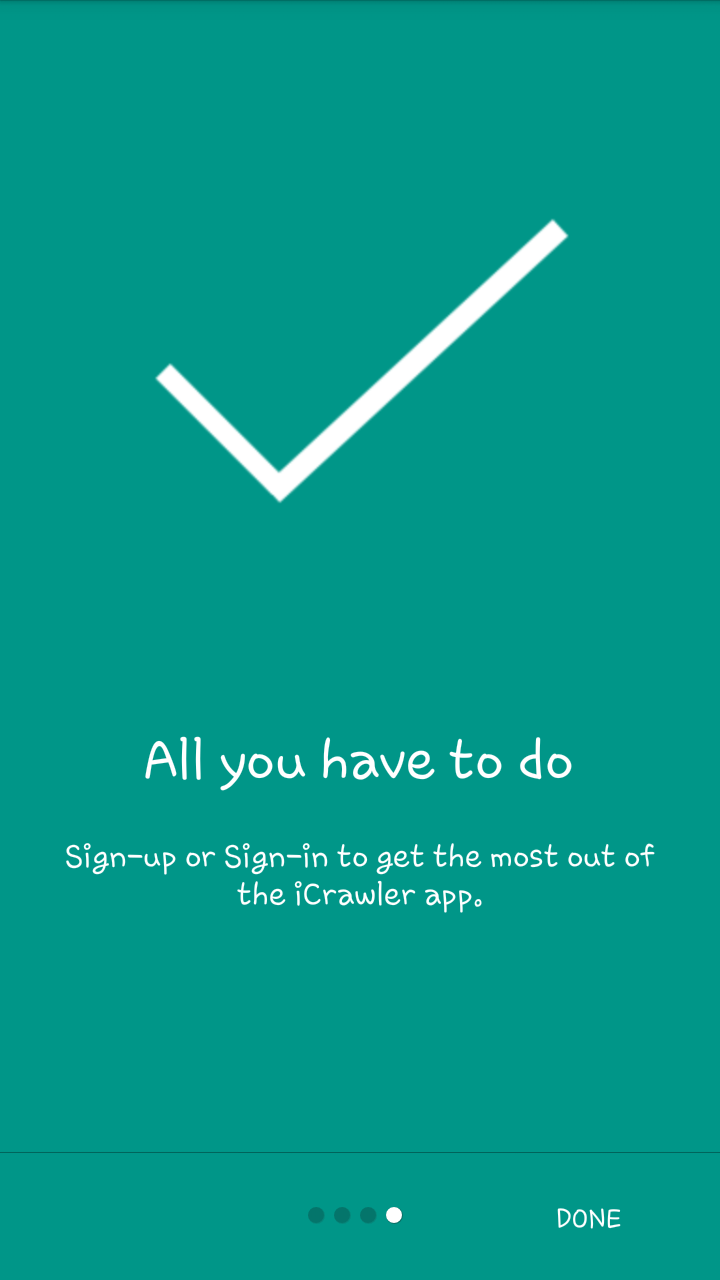
\includegraphics[width=0.5 \textwidth]{img/newImgs/tourThree.png}
	 	 \end{figure}\newpage	 	 
	 	 
	 	\item \textbf{Skip tour}\newline
	 	If you decided to skip the app tour then you get the options to Sign up or Sign in; you can still take the tour by clicking the 
	 	'Take Tour' link at the bottom.\newline
	 	By signing up or signing in, you agree to our Terms and Privacy Policy. 
	 	 
	 	 %sign up%
	 	 \begin{figure}[h!]
	 	 	\caption{Signing up}
	 	 	\centering 																																		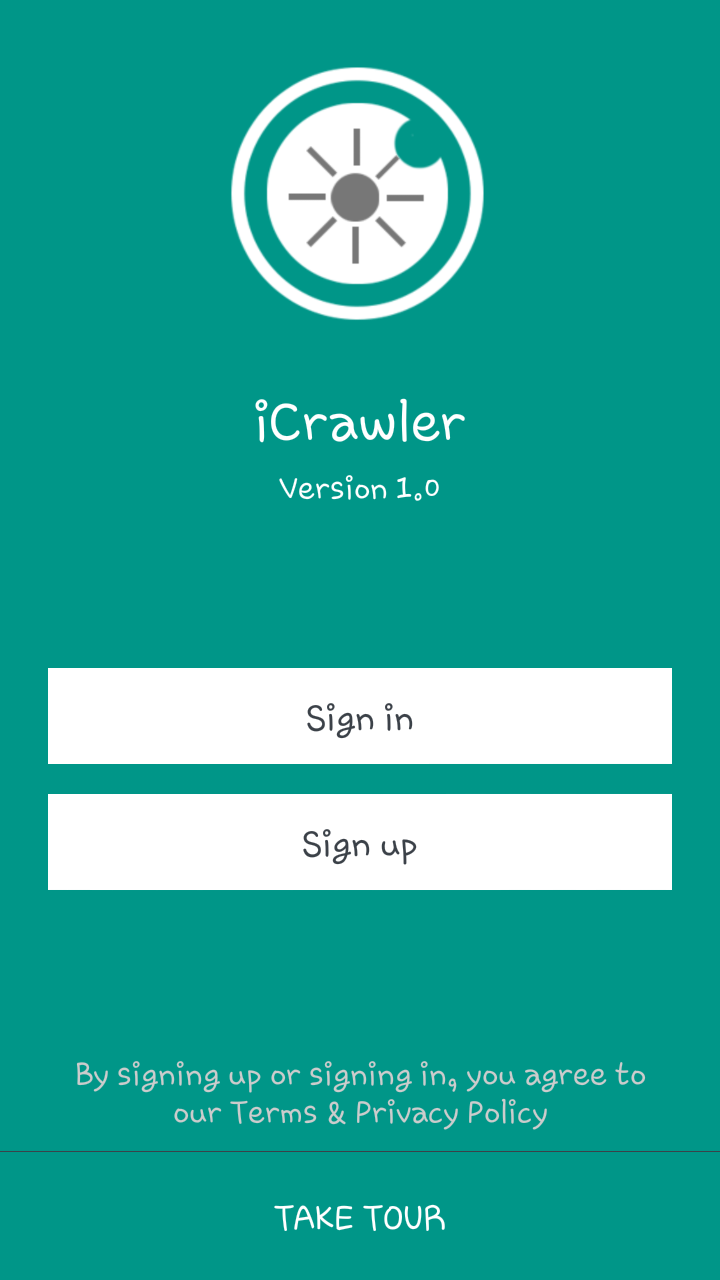
\includegraphics[width=0.5 \textwidth]{img/newImgs/homePage.png}
	 	 \end{figure}\newpage
	 	 
	 	 If you have never used the iCrawler app before, you need to sign up; simply enter your valid email address and password then
	 	click the 'orange arrow' pointing to the right in order to subscribe as a new user.
	 	
		%sign up%
	 	 \begin{figure}[h!]
	 	 	\caption{Signing up}
	 	 	\centering 																																		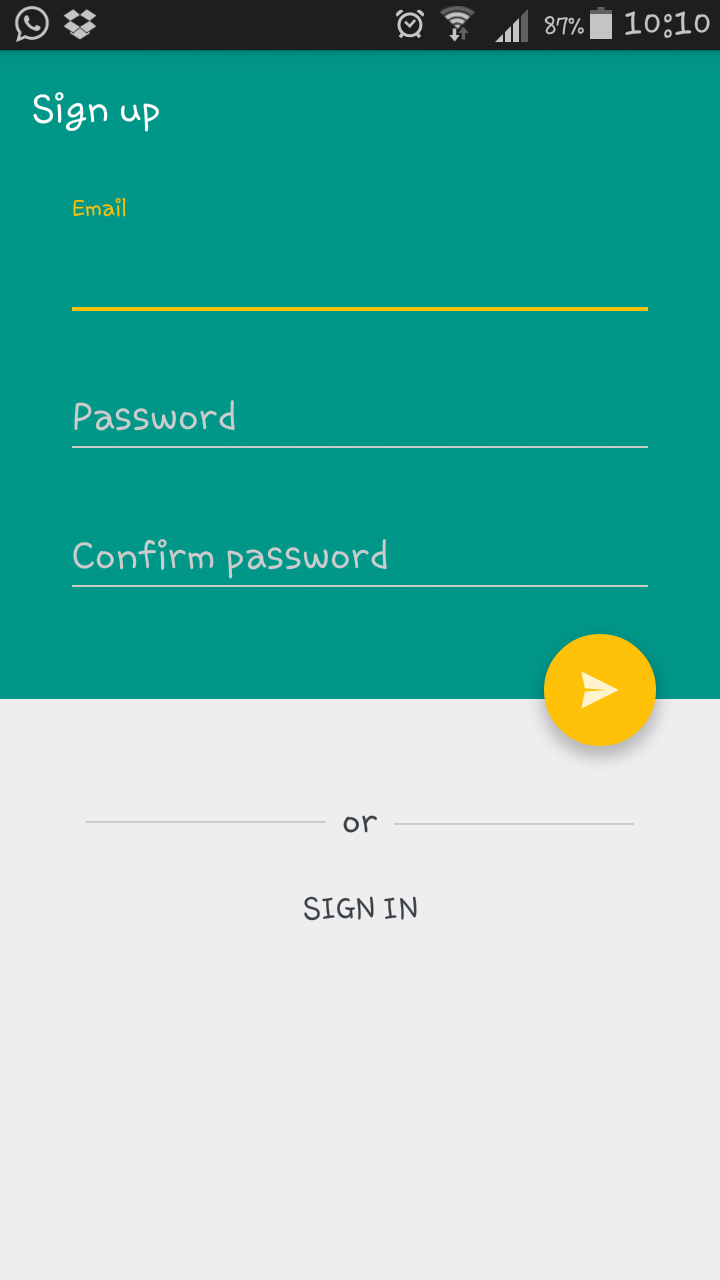
\includegraphics[width=0.5 \textwidth]{img/newImgs/signUp.png}
	 	 \end{figure}\newpage	 	 
	 	 
	 	If you have used the iCrawler app before, you need not to sign up again, simply enter your credentials and then
	 	click the 'orange arrow' pointing to the right in order to subscribe the new device. If not, click 'Sign up' to register as a new user.
	 	
	 	%sign in%
	 	 \begin{figure}[h!]
	 	 	\caption{Signing in}
	 	 	\centering 																																		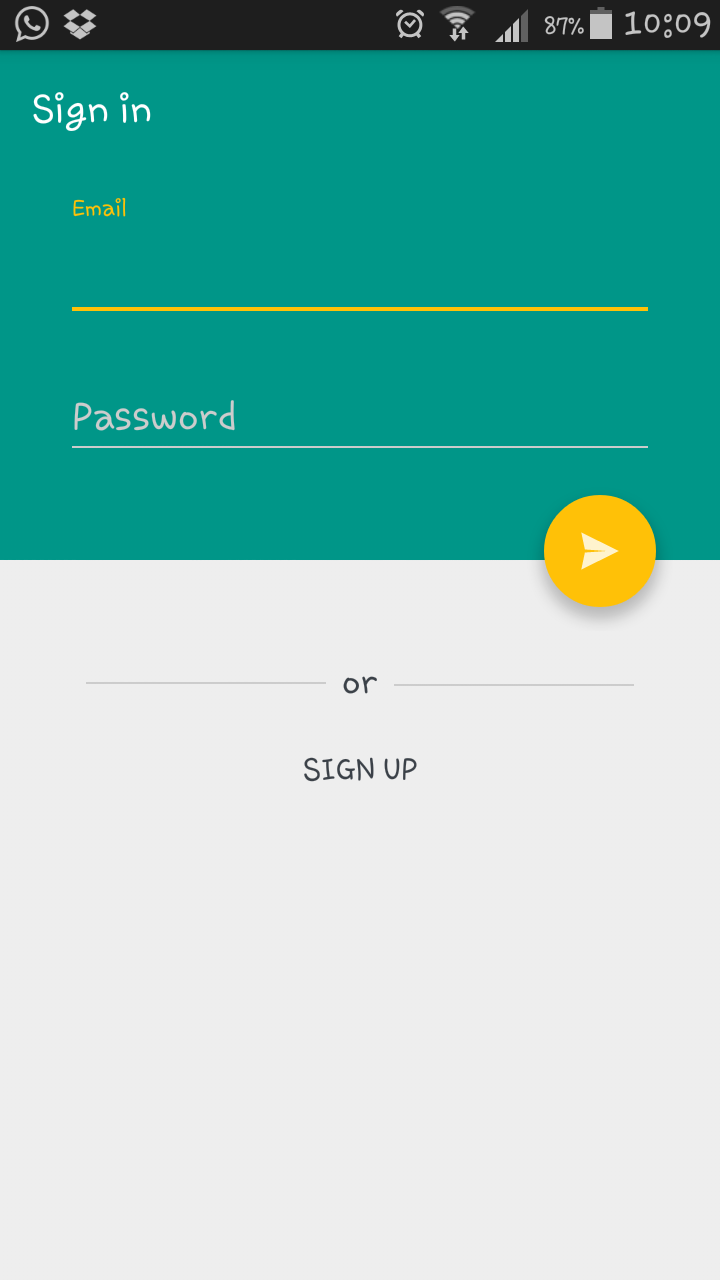
\includegraphics[width=0.5 \textwidth]{img/newImgs/signIn.png}
	 	 \end{figure}
	 	 
	 \end{itemize}\newpage
	 
	 
	\section{Using the Mobile App}
	The app runs in the background after 'Signing up' or 'Signing in'; there is no other form of interaction with 
	the app thereafter. You can access the log reports generated via the web application (dashboard).
	\newline\newline
	
	\section{Using the Web App}
	The data collected from the mobile device can only be viewed using the web application (dashboard). The dashboard is highly responsive to different window dimensions but we recommend not going below 700x800. 
	
	\begin{itemize}
		%%%%%%%%%%%%%%%%%%%%% start %%%%%%%%%%%%%%%%%%%%%%%%%%%%%%%%
	 	\item \textbf{Landing page}\newline
	 	This is the landing page that appears when using the desktop web browser. To login, the user must provide the requested credentials, which are the same as the ones he/she used when 'signing up' or 'signing in' using the mobile device app.
	 	 
	 	 %Welcome page%
	 	 \begin{figure}[h!]
	 	 	\caption{Login page}
	 	 	\centering 																																		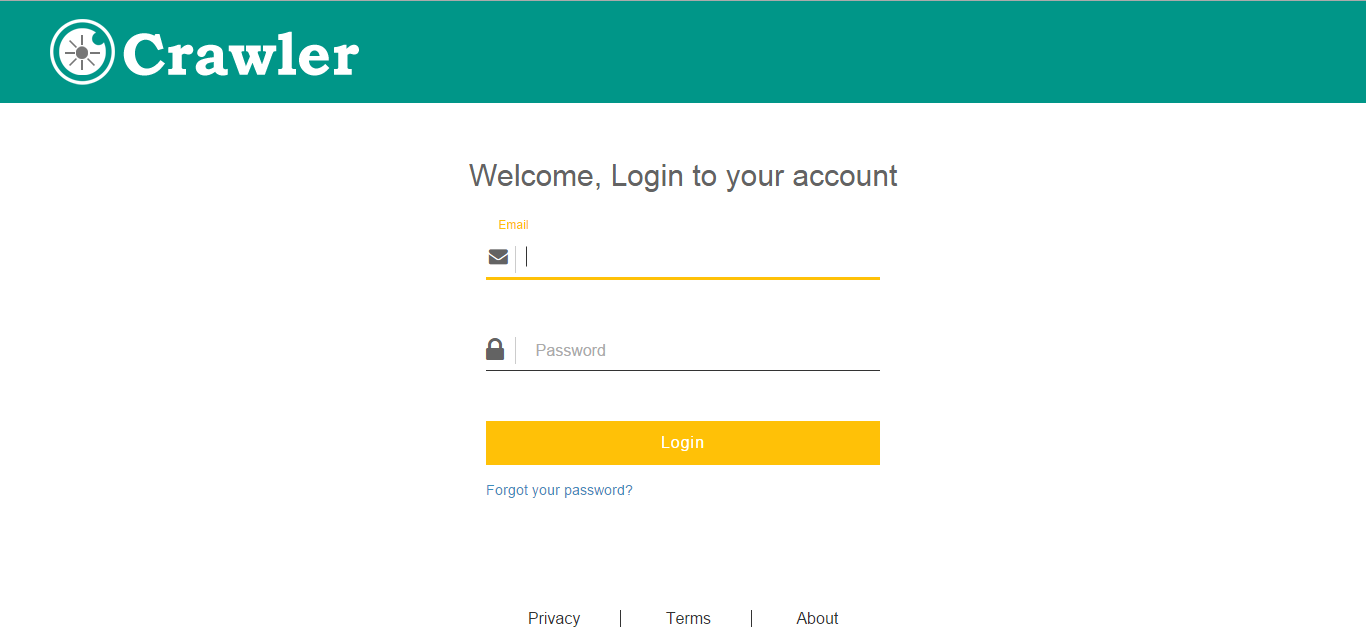
\includegraphics[width=1 \textwidth]{img/dashboard/loginPage.png}
	 	 \end{figure}\newpage
	 	 
	 	 %%%%%%%%%%%%%%%%%%%%% start %%%%%%%%%%%%%%%%%%%%%%%%%%%%%%%%
		\item \textbf{Home page}\newline
	 	On successful login, the user is welcomed by the dashboard home page.\newline
	 	This page summarizes the data collected from the devices and all the devices linked with the current user account. On the top-left you find a notifier informing the user about the currently selected device and whether or not the device is on(green)/off(red).
	 	 
	 	 %dashboard home%
	 	 \begin{figure}[h!]
	 	 	\caption{Dashboard control panel}
	 	 	\centering 																																		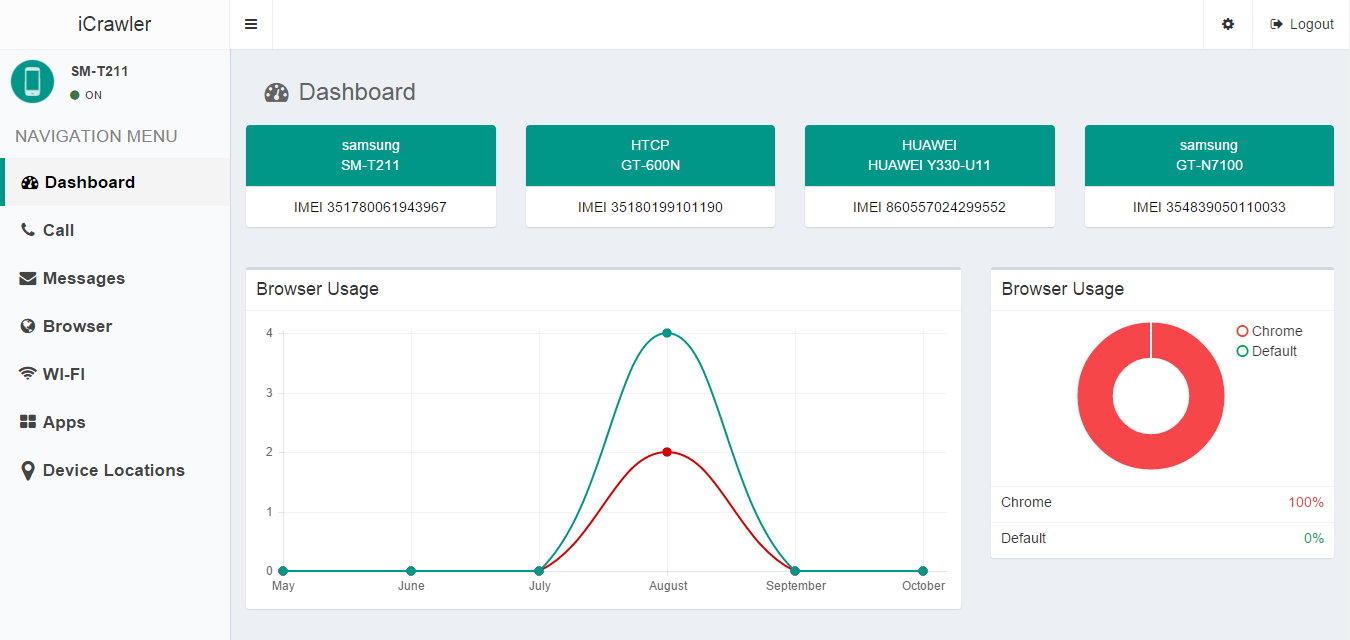
\includegraphics[width=1 \textwidth]{img/dashboard/dashboardLandingPage.png}
	 	 \end{figure}\newpage	
	 	 
	 	 %%%%%%%%%%%%%%%%%%%%% start %%%%%%%%%%%%%%%%%%%%%%%%%%%%%%%%
	 	 \item \textbf{Calls page}\newline
	 	This page consists of the reports collected from the call activities on the mobile device. A summary of the total dialed, received, and missed calls is provided to aid the user.
	 	 
	 	 %calls home%
	 	 \begin{figure}[h!]
	 	 	\caption{Call data}
	 	 	\centering 																																		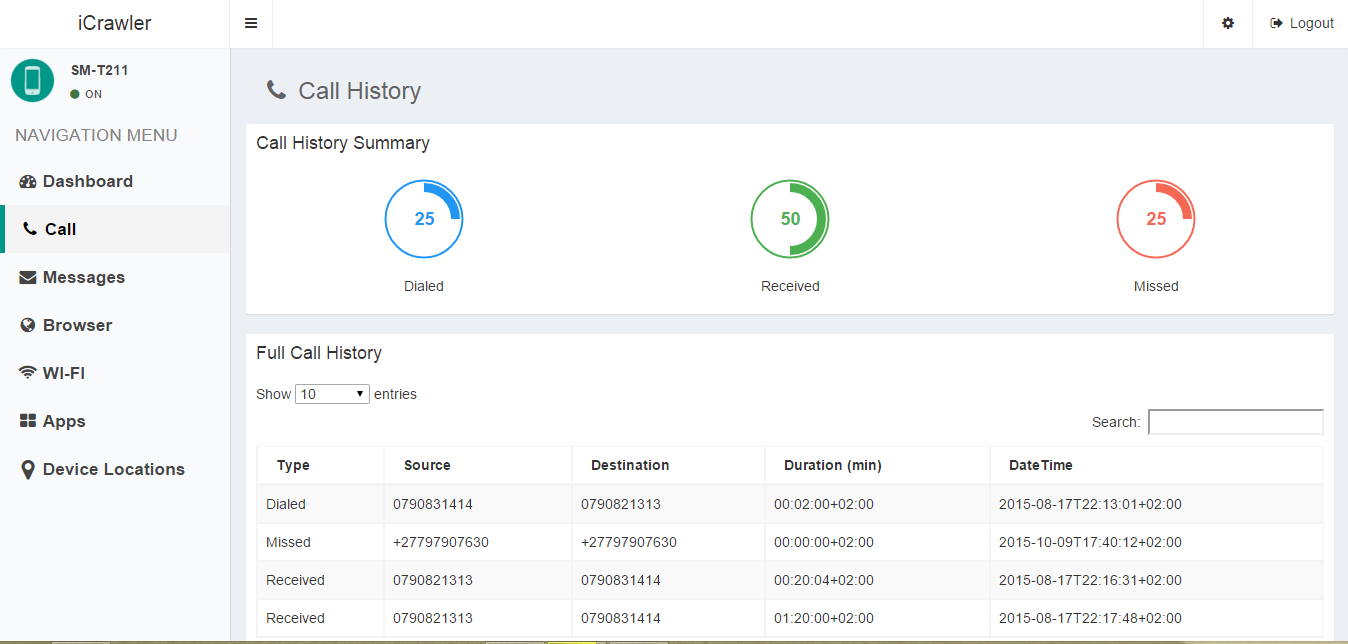
\includegraphics[width=1 \textwidth]{img/dashboard/dashboardCall.png}
	 	 \end{figure}\newpage	
	 	 
	 	 %%%%%%%%%%%%%%%%%%%%% start %%%%%%%%%%%%%%%%%%%%%%%%%%%%%%%%
	 	 \item \textbf{Messages page}\newline
	 	This page consists of the reports collected from the messaging activities on the mobile device. Due to the Privacy Act in our country we can not retrieve the communicated content.
	 	 
	 	 %messages home%
	 	 \begin{figure}[h!]
	 	 	\caption{Messages data}
	 	 	\centering 																																		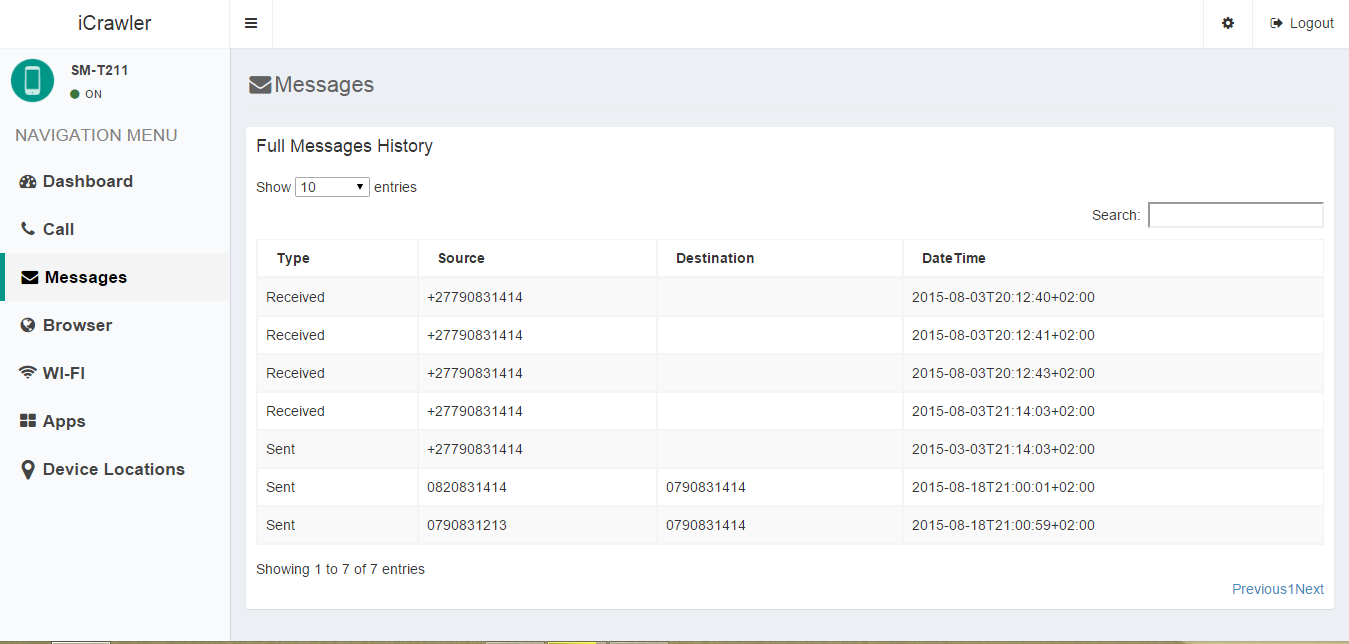
\includegraphics[width=1 \textwidth]{img/dashboard/dashboardMessages.png}
	 	 \end{figure}\newpage	
	 
	 %%%%%%%%%%%%%%%%%%%%% start %%%%%%%%%%%%%%%%%%%%%%%%%%%%%%%%
	 	 \item \textbf{Browser page}\newline
	 	This page consists of the reports collected from the internet browsing activities on the mobile device. The browser used, URL visited, including the frequency are included in the report.
	 	 
	 	 %browser home%
	 	 \begin{figure}[h!]
	 	 	\caption{Internet browsing data}
	 	 	\centering 																																		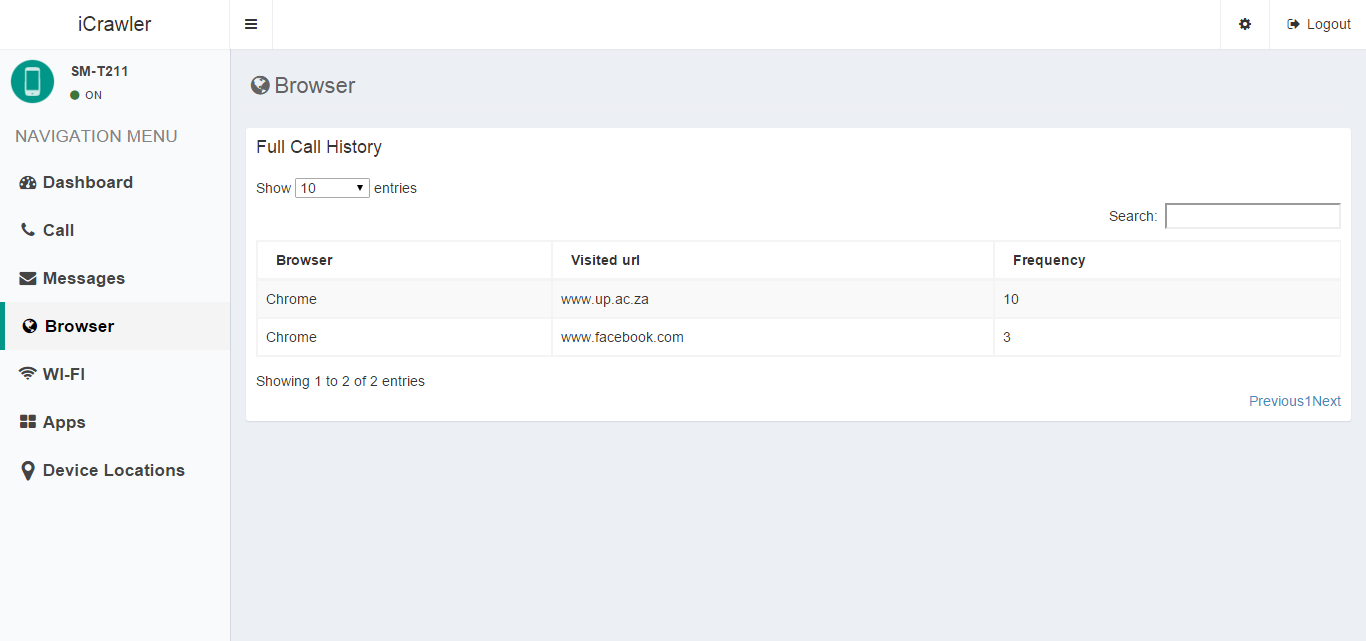
\includegraphics[width=1 \textwidth]{img/dashboard/dashboardBrowser.png}
	 	 \end{figure}\newpage	
	 	 
	 	 %%%%%%%%%%%%%%%%%%%%% start %%%%%%%%%%%%%%%%%%%%%%%%%%%%%%%%
	 	 \item \textbf{Wifi page}\newline
	 	This page consists of the reports collected from the wifi connection activities on the mobile device. 
	 	 
	 	 %wifi home%
	 	 \begin{figure}[h!]
	 	 	\caption{Wifi connection data}
	 	 	\centering 																																		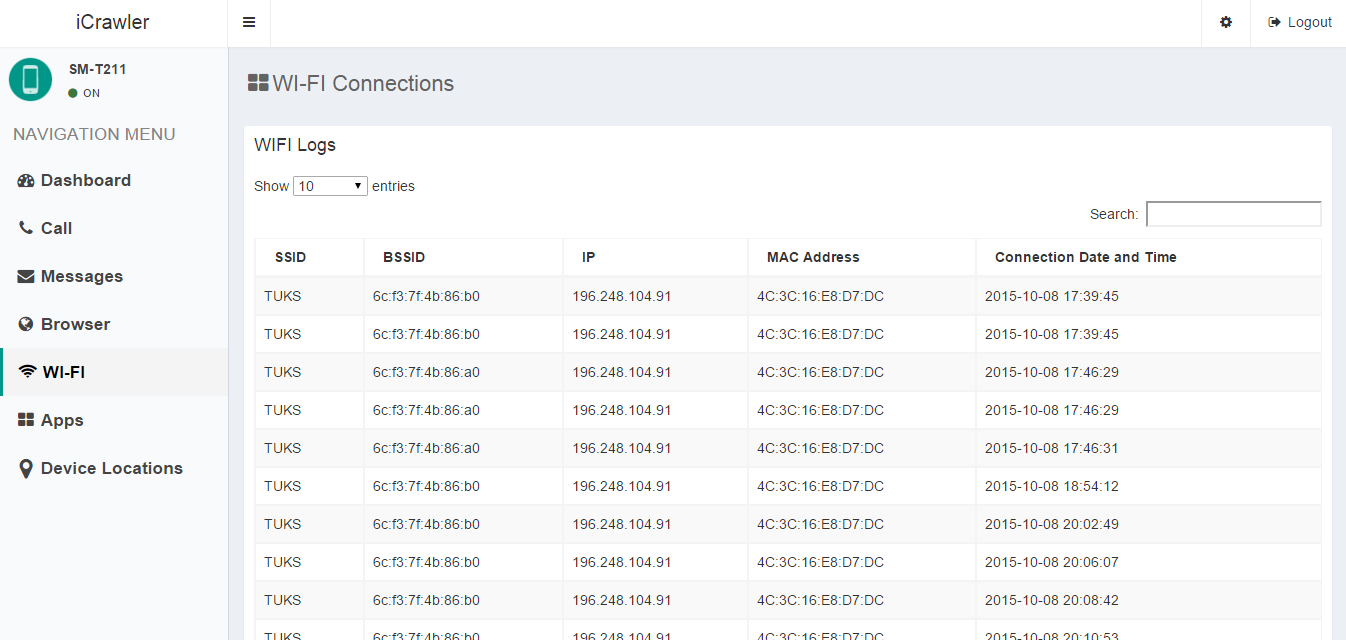
\includegraphics[width=1 \textwidth]{img/dashboard/dashboardWifi.png}
	 	 \end{figure}\newpage
	 	 
	 	 %%%%%%%%%%%%%%%%%%%%% start %%%%%%%%%%%%%%%%%%%%%%%%%%%%%%%%
	 	 \item \textbf{Apps page}\newline
	 	This page consists of the reports collected from the installed apps on the mobile device. The 'running status' column assists in determining whether the app runs on the foreground, running or stopped/closed.
	 	 
	 	 %apps home%
	 	 \begin{figure}[h!]
	 	 	\caption{Installed apps data}
	 	 	\centering 																																		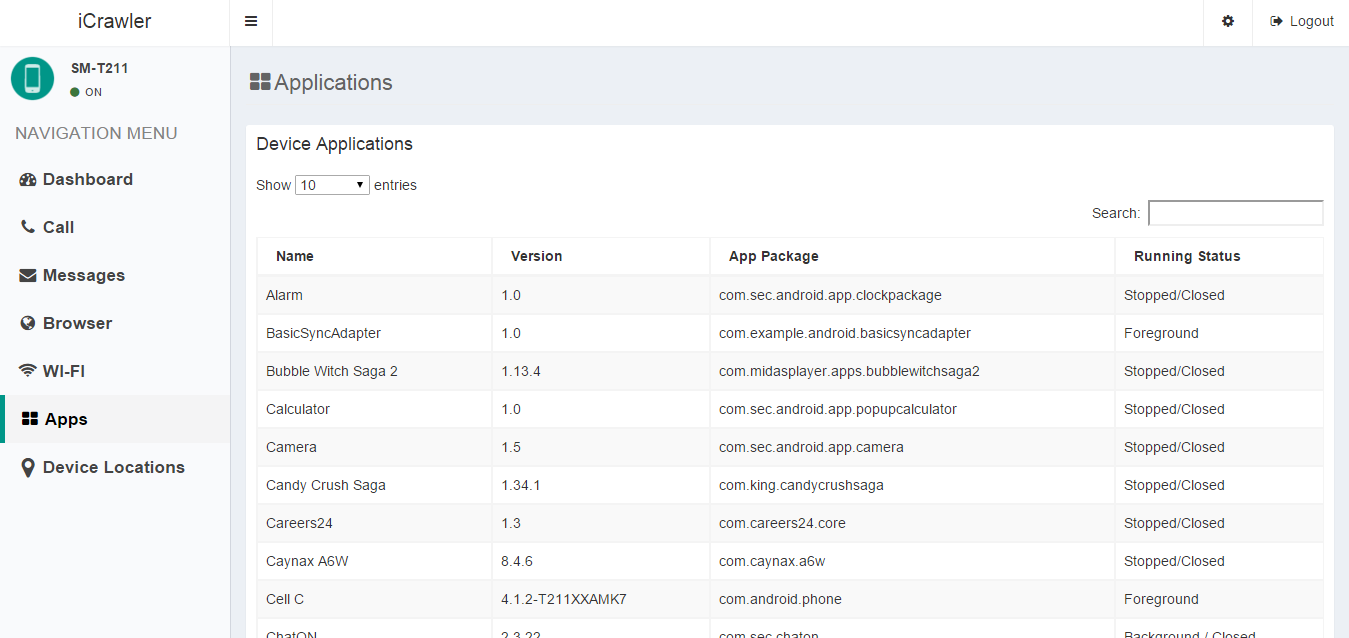
\includegraphics[width=1 \textwidth]{img/dashboard/dashboardApp.png}
	 	 \end{figure}\newpage	
	 	 
	 	 %%%%%%%%%%%%%%%%%%%%% start %%%%%%%%%%%%%%%%%%%%%%%%%%%%%%%%
	 	 \item \textbf{Device location page}\newline
	 	This page consists of a summary of the last know locations of the user's mobile device. This data is reported every 30min. 
	 	 
	 	 %device location home%
	 	 \begin{figure}[h!]
	 	 	\caption{Geo location data}
	 	 	\centering 																																		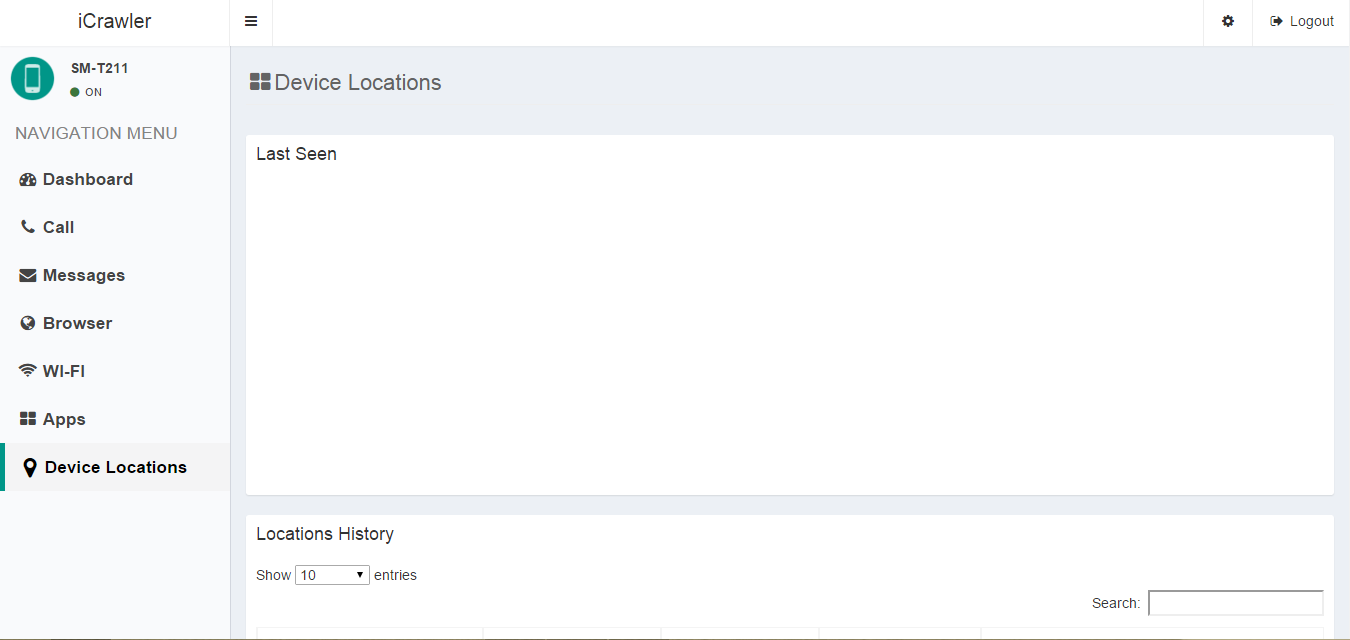
\includegraphics[width=1 \textwidth]{img/dashboard/dashboardDeviceLocations.png}
	 	 \end{figure}\newpage	
	 	 
	 	 %%%%%%%%%%%%%%%%%%%%% start %%%%%%%%%%%%%%%%%%%%%%%%%%%%%%%%
	 	 \item \textbf{Privacy page}\newline
	 	The privacy policy of the iCrawler services are all stated here. 
	 	 
	 	 %privacy home%
	 	 \begin{figure}[h!]
	 	 	\caption{Privacy policy}
	 	 	\centering 																																		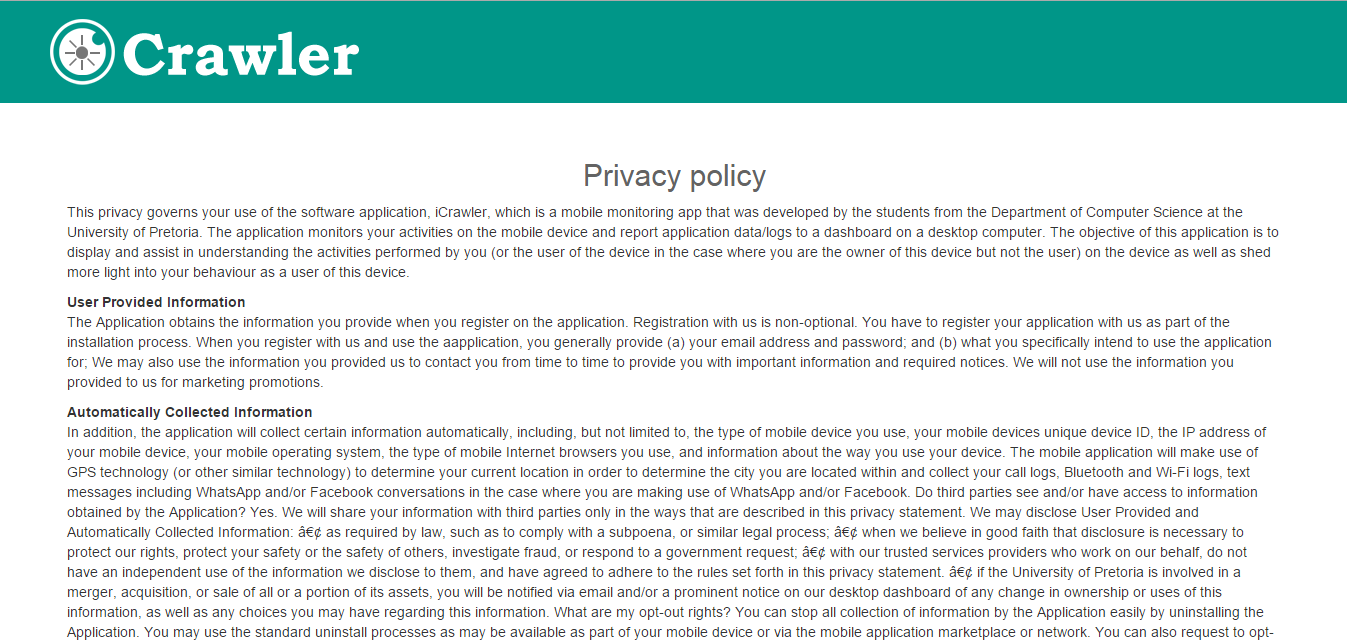
\includegraphics[width=1 \textwidth]{img/dashboard/privacy.png}
	 	 \end{figure}\newpage	
	 	 
	 	 	 	 %%%%%%%%%%%%%%%%%%%%% start %%%%%%%%%%%%%%%%%%%%%%%%%%%%%%%%
	 	 \item \textbf{Terms page}\newline
	 	The Terms of use of the iCrawler services are all stated here. 
	 	 
	 	 %terms home%
	 	 \begin{figure}[h!]
	 	 	\caption{Terms of use}
	 	 	\centering 																																		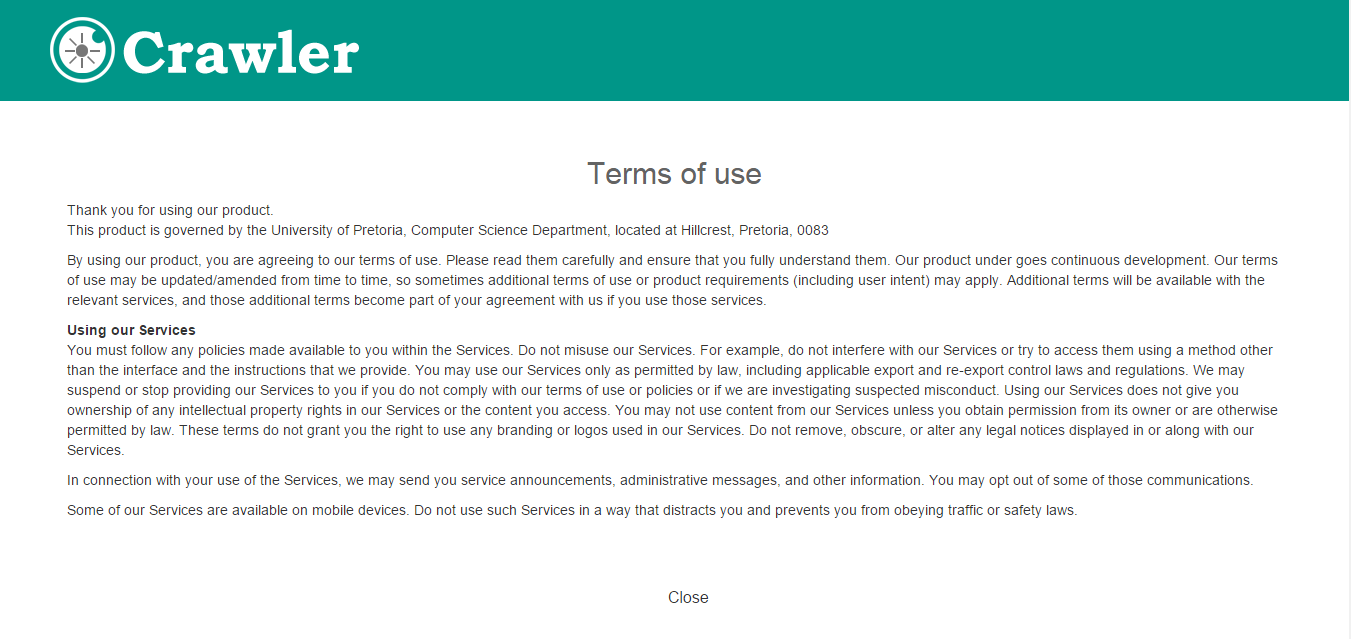
\includegraphics[width=1 \textwidth]{img/dashboard/termsAndUse.png}
	 	 \end{figure}\newpage	
	 	 
	 	 	 	 %%%%%%%%%%%%%%%%%%%%% start %%%%%%%%%%%%%%%%%%%%%%%%%%%%%%%%
	 	 \item \textbf{About page}\newline
	 	This About page consists of all the relevant information regarding all the involved parties in this project. 
	 	 
	 	 %about home%
	 	 \begin{figure}[h!]
	 	 	\caption{About us}
	 	 	\centering 																																		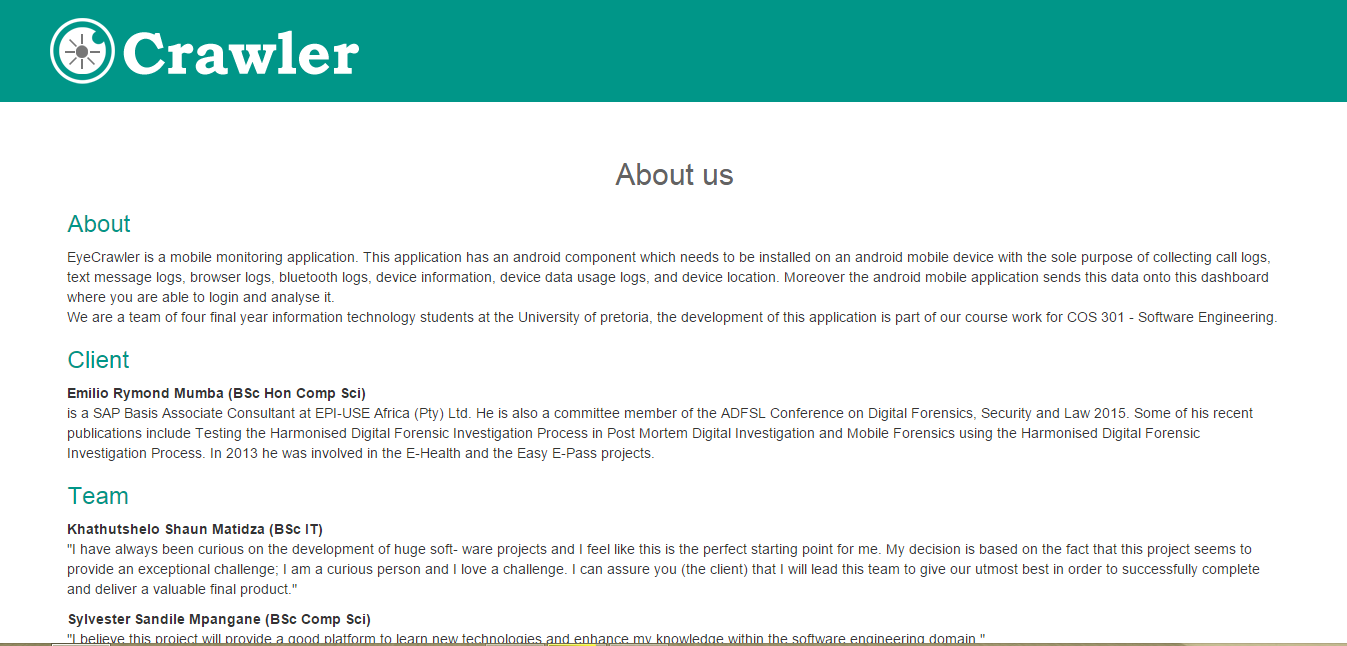
\includegraphics[width=1 \textwidth]{img/dashboard/aboutUs.png}
	 	 \end{figure}\newpage	
	 	 
	 \end{itemize}
	%%%%%%%%%%%%%%%%%%%%end of Dashboard section%%%%%%%%%%%%%%%%%%%%%%%%%%
	
	\section{Troubleshooting}
	The following section lists some of the iCrawler app's possible issues and resolutions:
	
	\begin{itemize}
		\item \textbf{Does not launch.} Restart your phone and try to launch the application again.
		\item\textbf{Crashes immediately after launch.} Ensure that your device meets the minimum specifications to run
		 iCrawler (See configurations). Go to Settings $\rightarrow$ Apps $\rightarrow$ Manage Apps $\rightarrow$ Running, to check if your apps are not using up all
		  your memory. Try to end all processes you do not need and re-start your phone.
		\item \textbf{Other unknown causes.} If problems continue, delete the app completely and then reinstall it.\
	\end{itemize}
		
\end{document}
